\documentclass[11pt,a4paper]{ctexart}
\usepackage[student]{ipara}
\usepackage{paracol}
\usepackage{mathtools}
\usetikzlibrary{calc,arrows.meta,positioning}

\definecolor{rulecolor}{RGB}{90,105,125}
\definecolor{teachblue}{RGB}{32,91,161}
\definecolor{softblue}{RGB}{239,246,253}
\definecolor{softgray}{RGB}{247,248,250}
\definecolor{softorange}{RGB}{255,247,235}

% Parallel-projection basis used by the major 3D figures.
\tikzset{spatial/.style={
  x={(0.95cm,-0.10cm)},
  y={(0.48cm,0.34cm)},
  z={(0cm,0.88cm)},
  >=Stealth,line join=round,line cap=round
}}

% =====================================================
% 页眉页脚设置
% =====================================================
\pagestyle{fancy}
\fancyhf{}
\lhead{\small 公共专题学案：立体几何——线面平行垂直与书写规范}
\rhead{\small 学生版}
\cfoot{\small 第 \thepage\ 页\quad 共 \zpageref{LastPage} 页}
\renewcommand{\headrulewidth}{0.4pt}
\renewcommand{\footrulewidth}{0pt}

% =====================================================
% 公式准备（含默写控制）
% =====================================================
\newcommand{\sessionformulas}{%
  \arrayrulecolor{rulecolor}
  \begin{tabularx}{\textwidth}{p{4.0cm}X}
  \toprule[1.2pt]
  线面平行判定 & 若 $m\subset\alpha$，$l\parallel m$，且 \fblank[2.2cm]{$l\not\subset\alpha$}，则 $l\parallel\alpha$。\\ \hline
  线面平行性质 & 若 $l\parallel\alpha$，$l\subset\beta$，$\alpha\cap\beta=m$，则 \fblank[2.2cm]{$l\parallel m$}。\\ \hline
  面面平行判定 & 若 $a,b\subset\beta$，\fblank[2.2cm]{$a\cap b=O$}，且 $a\parallel\alpha$，$b\parallel\alpha$，则 $\beta\parallel\alpha$。\\ \hline
  线面垂直判定 & 若 $a,b\subset\alpha$，\fblank[2.2cm]{$a\cap b=O$}，且 $l\perp a$，$l\perp b$，则 $l\perp\alpha$。\\ \hline
  线面垂直性质 & 若 $l\perp\alpha$，$a\subset\alpha$，则 \fblank[2.2cm]{$l\perp a$}。\\ \hline
  面面垂直判定 & 若 $l\subset\beta$，\fblank[2.2cm]{$l\perp\alpha$}，则 $\beta\perp\alpha$。\\ \hline
  面面垂直性质 & 若 $\alpha\perp\beta$，$\alpha\cap\beta=m$，$l\subset\alpha$，\fblank[2.2cm]{$l\perp m$}，则 $l\perp\beta$。\\ \hline
  二级结论 & 若 $\alpha\perp\gamma$，$\beta\perp\gamma$，$\alpha\cap\beta=l$，则 \fblank[2.2cm]{$l\perp\gamma$}。\\ \hline
  核心防错提炼 & 证明线面垂直时，必须说明两条直线 \fblank[2.5cm]{在目标平面内且相交}；证明线面平行时，必须排除 \fblank[2.5cm]{直线在平面内}。\\
  \bottomrule[1.2pt]
  \end{tabularx}
}

% =====================================================
\begin{document}

\begin{center}
  {\Large\bfseries 立体几何——线面平行垂直与书写规范}\par
  \vspace{0.3em}
  {\large 专题学案：把空间关系翻译成可得分的证明链}\par
  \vspace{0.3em}
  姓名：\blank{2.6cm}
  \quad
  日期：\blank{2.6cm}
  \quad
  时长：120 分钟
\end{center}

% =====================================================
% 第一板块：核心观念与基本定理
% =====================================================
\section{核心观念与基本定理}

\begingroup
\large
\renewcommand{\arraystretch}{1.55}
\linespread{1.35}\selectfont
\showpromptfalse
\sessionformulas
\endgroup

\vspace{0.8em}
\begin{tcolorbox}[enhanced,breakable,colback=white,colframe=rulecolor,boxrule=0.55pt,arc=1mm,left=1.4mm,right=1.4mm,top=1.1mm,bottom=1.1mm,title={看到条件，立刻想到什么},fonttitle=\bfseries]
\begin{itemize}[leftmargin=2em, itemsep=0.1em]
  \item 看到“证明线面平行” $\to$ 在目标平面内找一条与已知直线平行的直线。
  \item 看到“证明面面平行” $\to$ 在一个平面内找两条相交直线，分别平行于另一个平面。
  \item 看到“中点”“三等分点” $\to$ 中位线、平行四边形、相似或向量比例。
  \item 看到“证明线线垂直” $\to$ 先证明其中一条线垂直于某个平面。
  \item 看到“证明面面垂直” $\to$ 在一个平面内找一条线垂直于另一个平面。
  \item 看到“两个平面垂直且给出交线” $\to$ 在一个平面内找垂直交线的直线，推出它垂直另一个平面。
\end{itemize}
\end{tcolorbox}

\newpage

% =====================================================
% 第二板块：应试书写规范
% =====================================================
\section{应试书写规范：先把“得分句”定下来}

\begin{tcolorbox}[enhanced,breakable,colback=white,colframe=rulecolor,boxrule=0.55pt,arc=1mm,left=1.4mm,right=1.4mm,top=1.1mm,bottom=1.1mm,title={核心要求：看出来不等于证明出来},fonttitle=\bfseries]
证明题本质是写成阅卷老师可识别的完整逻辑链。下面每一个标准的得分句前提，都必须在解答中写全。
\end{tcolorbox}

\vspace{0.4em}
\begin{tabularx}{\textwidth}{p{3.2cm}X}
\toprule
目标 & 标准得分句 / 必查前提 \\
\midrule
线面平行 & $m\subset\alpha,\ l\parallel m,\ l\not\subset\alpha\Rightarrow l\parallel\alpha$。最容易漏：$l\not\subset\alpha$。 \\ \hline
线面垂直 & $a,b\subset\alpha,\ a\cap b=O,\ l\perp a,\ l\perp b\Rightarrow l\perp\alpha$。最容易漏：$a,b$ 在目标平面内且相交。 \\ \hline
面面平行 & 在同一平面内找两条相交直线，分别与另一平面平行；或分别平行于另一平面内两条相交直线。 \\ \hline
面面垂直 & 在其中一个平面内找到一条直线 $l$，证明 $l\perp$ 另一个平面。 \\ \hline
面面垂直性质 & 必须写出交线：$\alpha\perp\beta,\ \alpha\cap\beta=m,\ l\subset\alpha,\ l\perp m\Rightarrow l\perp\beta$。 \\
\bottomrule
\end{tabularx}
\vspace{0.6em}

\begin{tcolorbox}[colback=softblue,colframe=teachblue,boxrule=0.7pt,arc=1.2mm,left=1.4mm,right=1.4mm,top=1.2mm,bottom=1.2mm,title={四步自查：每次写完证明后都扫一遍},fonttitle=\bfseries]
\begin{enumerate}[label=\arabic*. , leftmargin=2em, itemsep=0.1em]
  \item \textbf{归属}：关键直线是否明确写了属于哪个平面？
  \item \textbf{相交}：线面垂直、面面平行中用到的两条直线是否明确相交？
  \item \textbf{排除}：证明线面平行时，是否排除了直线在平面内？
  \item \textbf{定理链}：每一个“所以”前面，是否已经凑齐对应定理的全部前提？
\end{enumerate}
\end{tcolorbox}

\newpage

% =====================================================
% 第三板块：选择题易错判断（6 道核心题）
% =====================================================
\section{选择题易错判断}

\begin{choiceblock}

% --- 选择 1 ---
\automcfigurequestion{已知互相垂直的两个平面 $\alpha,\beta$ 交于直线 $l$，若直线 $m$ 满足 $m\perp\alpha$，则下列结论正确的是}{
  \mcoptions{$m\perp\beta$}{$m\perp l$}{$m\parallel\beta$}{$m\parallel l$}
}{
  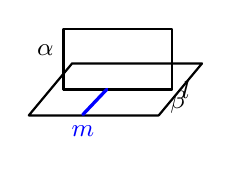
\begin{tikzpicture}[scale=0.55,>=Stealth,line join=round,line cap=round]
    \draw[thick] (0,0)--(3.0,0)--(4.0,1.2)--(1.0,1.2)--cycle;
    \node at (3.45,0.3){\small $\beta$};
    \draw[thick] (0.8,0.6)--(3.3,0.6)--(3.3,2.0)--(0.8,2.0)--cycle;
    \node[left] at (0.8,1.5){\small $\alpha$};
    \draw[thick] (0.8,0.6)--(3.3,0.6) node[right]{\small $l$};
    \coordinate(F) at (1.8,0.6);
    \draw[very thick,blue] (F)--(1.25,0.02) node[below]{\small $m$};
  \end{tikzpicture}
}
\choiceworkarea[3.2cm]

% --- 选择 2 ---
\automcfigurequestion{设 $\alpha,\beta$ 是互不重合的平面，$l,m,n$ 是互不重合的直线，下列命题正确的是}{
  \mcoptions{若 $m,n\subset\alpha$，$l\perp m$，$l\perp n$，则 $l\perp\alpha$}{若 $l\perp m$，$l\perp n$，则 $m\parallel n$}{若 $l\parallel\alpha$，$m\parallel\beta$，$\alpha\perp\beta$，则 $l\perp m$}{若 $l\perp\alpha$，$l\parallel\beta$，则 $\alpha\perp\beta$}
}{
  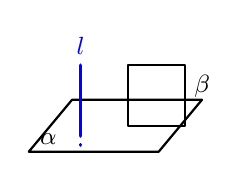
\begin{tikzpicture}[scale=0.55,>=Stealth,line join=round,line cap=round]
    \draw[thick] (0,0)--(3.0,0)--(4.0,1.2)--(1.0,1.2)--cycle;
    \node at (0.45,0.3){\small $\alpha$};
    \draw[thick] (2.3,0.6)--(2.3,2.0)--(3.6,2.0)--(3.6,0.6)--cycle;
    \node[right] at (3.6,1.5){\small $\beta$};
    \draw[very thick,blue] (1.2,0.55)--(1.2,2.0) node[above]{\small $l$};
    \draw[dashed,very thick,blue] (1.2,0.55)--(1.2,0.15);
  \end{tikzpicture}
}
\choiceworkarea[4.5cm]

% --- 选择 3 ---
\automcfigurequestion{已知 $a,b,c$ 为三条不重合的直线，$\alpha,\beta,\gamma$ 为三个不重合的平面。\newline
(1) $a\parallel c,\ b\parallel c\Rightarrow a\parallel b$；\quad
(2) $a\parallel\gamma,\ b\parallel\gamma\Rightarrow a\parallel b$；\newline
(3) $a\parallel c,\ c\parallel\alpha\Rightarrow a\parallel\alpha$；\quad
(4) $a\parallel\gamma,\ a\parallel\alpha\Rightarrow\alpha\parallel\gamma$；\newline
(5) $a\not\subset\alpha,\ b\subset\alpha,\ a\parallel b\Rightarrow a\parallel\alpha$。其中正确命题为}{
  \mcoptions{(1)(5)}{(1)(2)(5)}{(1)(3)(5)}{(3)(4)(5)}
}{
  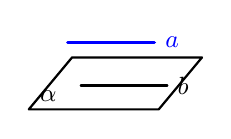
\begin{tikzpicture}[scale=0.55,>=Stealth,line join=round,line cap=round]
    \draw[thick] (0,0)--(3.0,0)--(4.0,1.2)--(1.0,1.2)--cycle;
    \node at (0.45,0.3){\small $\alpha$};
    \draw[thick] (1.2,0.55)--(3.2,0.55) node[right]{\small $b$};
    \draw[very thick,blue] (0.9,1.55)--(2.9,1.55) node[right]{\small $a$};
  \end{tikzpicture}
}
\choiceworkarea[4.5cm]

% --- 选择 4 ---
\automcfigurequestion{已知 $l\subset\alpha$，$\alpha\perp\beta$，$\alpha\cap\beta=m$。则“$l\perp m$”是“$l\perp\beta$”的}{
  \mcoptions{充分不必要条件}{必要不充分条件}{充要条件}{既不充分也不必要条件}
}{
  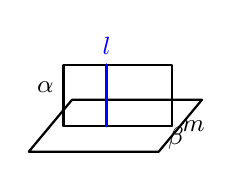
\begin{tikzpicture}[scale=0.55,>=Stealth,line join=round,line cap=round]
    \draw[thick] (0,0)--(3.0,0)--(4.0,1.2)--(1.0,1.2)--cycle;
    \node at (3.4,0.3){\small $\beta$};
    \draw[thick] (0.8,0.6)--(3.3,0.6)--(3.3,2.0)--(0.8,2.0)--cycle;
    \node[left] at (0.8,1.5){\small $\alpha$};
    \draw[thick] (0.8,0.6)--(3.3,0.6) node[right]{\small $m$};
    \draw[very thick,blue] (1.8,0.6)--(1.8,2.0) node[above]{\small $l$};
  \end{tikzpicture}
}
\choiceworkarea[3.5cm]

% --- 选择 5 ---
\automcfigurequestion{设 $m\subset\alpha$。则“$l\perp m$”是“$l\perp\alpha$”的}{
  \mcoptions{充分不必要条件}{必要不充分条件}{充要条件}{既不充分也不必要条件}
}{
  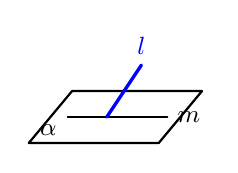
\begin{tikzpicture}[scale=0.55,>=Stealth,line join=round,line cap=round]
    \draw[thick] (0,0)--(3.0,0)--(4.0,1.2)--(1.0,1.2)--cycle;
    \node at (0.45,0.3){\small $\alpha$};
    \draw[thick] (0.9,0.6)--(3.2,0.6) node[right]{\small $m$};
    \draw[very thick,blue] (1.8,0.6)--(2.6,1.8) node[above]{\small $l$};
  \end{tikzpicture}
}
\choiceworkarea[3.5cm]

% --- 选择 6 ---
\automcfigurequestion{已知 $a,b$ 为两条不同直线，$\alpha,\beta$ 为两个不同平面，下列命题正确的是}{
  \mcoptions
  {若 $a\parallel b$，$a\parallel\alpha$，则 $b\parallel\alpha$}
  {若 $a\parallel b$，$a\perp\alpha$，$b\perp\beta$，则 $\alpha\perp\beta$}
  {若 $a\perp\alpha$，$b\perp\beta$，$\alpha\perp\beta$，则 $a\perp b$}
  {若 $a\parallel\alpha$，$b\parallel\beta$，$\alpha\perp\beta$，则 $a\perp b$}
}{
  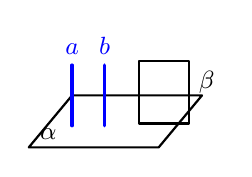
\begin{tikzpicture}[scale=0.55,>=Stealth,line join=round,line cap=round]
    \draw[thick] (0,0)--(3.0,0)--(4.0,1.2)--(1.0,1.2)--cycle;
    \node at (0.45,0.3){\small $\alpha$};
    \draw[thick] (2.55,0.55)--(2.55,2.0)--(3.7,2.0)--(3.7,0.55)--cycle;
    \node[right] at (3.7,1.5){\small $\beta$};
    \draw[very thick,blue] (1.0,0.5)--(1.0,1.9) node[above]{\small $a$};
    \draw[very thick,blue] (1.75,0.5)--(1.75,1.9) node[above]{\small $b$};
  \end{tikzpicture}
}
\choiceworkarea[4.0cm]

\end{choiceblock}

\newpage

% =====================================================
% 第四板块：平行证明代表性大题
% =====================================================
\section{平行证明代表性大题}

% --- 大题 1 ---
\freequestionheader
\noindent{\large\textbf{例 1\quad 四棱锥中证明 $EF\parallel$ 平面 $PAB$}}
\par\vspace{0.5em}

四棱锥 $P$-$ABCD$ 中，$AB\parallel CD$，$AB\perp AD$，且 $AB=AD=2CD=4$，$PA=2$，$\angle PAB=60^\circ$，直线 $PA$ 与平面 $ABCD$ 所成角为 $30^\circ$，$E,F$ 分别是 $BC$ 和 $PD$ 的中点。

求证：$EF\parallel$ 平面 $PAB$。

\begin{center}
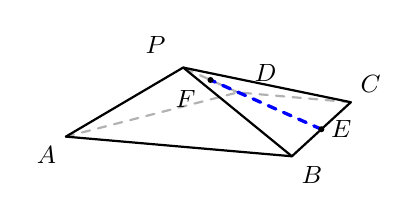
\begin{tikzpicture}[x={(0.92cm,-0.08cm)},y={(0.70cm,0.18cm)},z={(0cm,0.95cm)},>=Stealth,line join=round,line cap=round,scale=0.78]
  \coordinate (A) at (0,0,0);
  \coordinate (B) at (4,0,0);
  \coordinate (D) at (0,4,0);
  \coordinate (C) at (2,4,0);
  \coordinate (P) at (1,{sqrt(2)},1);
  \coordinate (E) at ($(B)!0.5!(C)$);
  \coordinate (F) at ($(P)!0.5!(D)$);

  \draw[dashed,thick,gray!60] (A)--(D)--(C);
  \draw[dashed,thick,gray!60] (D)--(P);
  \draw[thick] (A)--(B)--(C);
  \draw[thick] (A)--(P)--(B);
  \draw[thick] (P)--(C);

  \draw[very thick,blue,dashed] (E)--(F);

  \node[below left] at (A){\small $A$};
  \node[below right] at (B){\small $B$};
  \node[above right] at (C){\small $C$};
  \node[xshift=10pt,yshift=7pt] at (D){\small $D$};
  \node[xshift=-10pt,yshift=8pt] at (P){\small $P$};
  \fill (E) circle (1.4pt) node[right]{\small $E$};
  \fill (F) circle (1.4pt) node[xshift=-9pt,yshift=-7pt]{\small $F$};
\end{tikzpicture}
\end{center}

\answergrid[14cm]{证明：}

\newpage

% --- 大题 2 ---
\freequestionheader
\noindent{\large\textbf{例 2\quad 矩形底面中证明 $OE\parallel$ 平面 $PCD$}}
\par\vspace{0.5em}

四棱锥 $P$-$ABCD$ 中，四边形 $ABCD$ 是矩形，$\triangle PAD$ 是正三角形，且平面 $PAD\perp$ 平面 $ABCD$，$AB=1$。$O$ 为 $AD$ 的中点，$E$ 为 $PB$ 的中点。

求证：$OE\parallel$ 平面 $PCD$。

\begin{center}
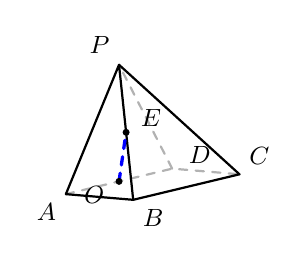
\begin{tikzpicture}[x={(0.95cm,-0.08cm)},y={(0.75cm,0.18cm)},z={(0cm,0.95cm)},>=Stealth,line join=round,line cap=round,scale=0.90]
  \coordinate (A) at (0,0,0);
  \coordinate (B) at (1,0,0);
  \coordinate (D) at (0,2,0);
  \coordinate (C) at (1,2,0);
  \coordinate (P) at (0,1,{sqrt(3)});
  \coordinate (O) at ($(A)!0.5!(D)$);
  \coordinate (E) at ($(P)!0.5!(B)$);

  \draw[dashed,thick,gray!60] (A)--(D)--(C);
  \draw[dashed,thick,gray!60] (D)--(P);
  \draw[thick] (A)--(B)--(C);
  \draw[thick] (A)--(P)--(B);
  \draw[thick] (P)--(C);

  \draw[very thick,blue,dashed] (O)--(E);

  \node[below left] at (A){\small $A$};
  \node[below right] at (B){\small $B$};
  \node[above right] at (C){\small $C$};
  \node[xshift=10pt,yshift=5pt] at (D){\small $D$};
  \node[xshift=-7pt,yshift=7pt] at (P){\small $P$};
  \fill (O) circle (1.4pt) node[xshift=-9pt,yshift=-5pt]{\small $O$};
  \fill (E) circle (1.4pt) node[xshift=9pt,yshift=5pt]{\small $E$};
\end{tikzpicture}
\end{center}

\answergrid[14cm]{证明：}

\newpage

% =====================================================
% 第五板块：垂直证明代表性大题
% =====================================================
\section{垂直证明代表性大题}

% --- 大题 3 ---
\freequestionheader
\noindent{\large\textbf{例 3\quad 平行四边形与面面垂直性质综合}}
\par\vspace{0.5em}

在四棱锥 $S$-$ABCD$ 中，平面 $SCD\perp$ 平面 $ABCD$，$SC=SD$。底面 $ABCD$ 是平行四边形，$\angle BAD=\frac{\pi}{3}$，$AB=2$，$AD=1$。$M,N$ 分别为线段 $CD,AB$ 的中点。

求证：$BD\perp$ 平面 $SMN$。

\begin{center}
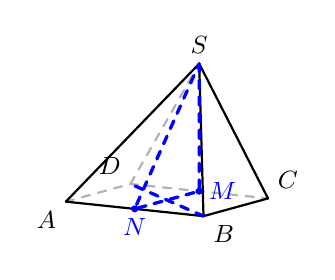
\begin{tikzpicture}[spatial,scale=0.92]
  \coordinate (A) at (0,0,0);
  \coordinate (B) at (2,0,0);
  \coordinate (D) at ({1/2},{sqrt(3)/2},0);
  \coordinate (C) at ({5/2},{sqrt(3)/2},0);
  \coordinate (M) at ({3/2},{sqrt(3)/2},0);
  \coordinate (N) at (1,0,0);
  \coordinate (S) at ({3/2},{sqrt(3)/2},2);

  \draw[dashed,thick,gray!60] (A)--(D)--(C);
  \draw[dashed,thick,gray!60] (D)--(S);
  \draw[thick] (A)--(B)--(C)--(S);
  \draw[thick] (A)--(S)--(B);

  \draw[very thick,blue,dashed] (B)--(D);
  \draw[very thick,blue,dashed] (S)--(M)--(N)--(S);

  \node[below left] at (A){\small $A$};
  \node[below right] at (B){\small $B$};
  \node[above right] at (C){\small $C$};
  \node[above left] at (D){\small $D$};
  \node[above] at (S){\small $S$};
  \fill[blue] (M) circle (1.4pt) node[right]{\small $M$};
  \fill[blue] (N) circle (1.4pt) node[below]{\small $N$};
\end{tikzpicture}
\end{center}

\answergrid[14cm]{证明：}

\newpage

% --- 大题 4 ---
\freequestionheader
\noindent{\large\textbf{例 4\quad 数量关系反推与综合线面垂直证明}}
\par\vspace{0.5em}

四棱锥 $P$-$ABCD$ 的底面 $ABCD$ 是边长为 $2$ 的正方形，平面 $PAB\perp$ 平面 $ABCD$，平面 $PAD\perp$ 平面 $ABCD$。$E$ 为 $PD$ 的中点，三棱锥 $P$-$ACE$ 的体积为 $\frac23$。

求证：$AE\perp$ 平面 $PCD$。

\begin{center}
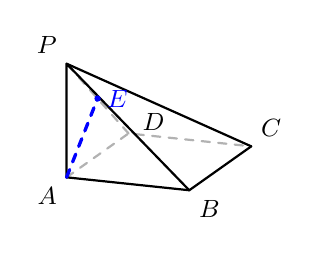
\begin{tikzpicture}[spatial,scale=0.82]
  \coordinate (A) at (0,0,0);
  \coordinate (B) at (2,0,0);
  \coordinate (D) at (0,2,0);
  \coordinate (C) at (2,2,0);
  \coordinate (P) at (0,0,2);
  \coordinate (E) at ($(P)!0.5!(D)$);

  \draw[dashed,thick,gray!60] (A)--(D)--(C);
  \draw[dashed,thick,gray!60] (D)--(P);
  \draw[thick] (A)--(B)--(C);
  \draw[thick] (A)--(P)--(B);
  \draw[thick] (P)--(C);
  \draw[very thick,blue,dashed] (A)--(E);

  \node[below left] at (A){\small $A$};
  \node[below right] at (B){\small $B$};
  \node[above right] at (C){\small $C$};
  \node[xshift=9pt,yshift=4pt] at (D){\small $D$};
  \node[above left] at (P){\small $P$};
  \fill[blue] (E) circle (1.4pt) node[right]{\small $E$};
\end{tikzpicture}
\end{center}

\answergrid[14cm]{证明：}

\newpage

% =====================================================
% 第六板块：公式默写关
% =====================================================
\section{公式默写关}

\begingroup
\large
\renewcommand{\arraystretch}{1.55}
\linespread{1.35}\selectfont
\showpromptfalse
\sessionformulas
\endgroup

% =====================================================
% 第七板块：课后重做与易错反思
% =====================================================
\section{课后重做与易错反思}

\begin{enumerate}[label=\arabic*. , leftmargin=2em, itemsep=1.1em]
  \item 第 \blank{1.2cm} 题：重做原因 \blank{5.5cm}

  \vspace{0.7cm}

  \item 第 \blank{1.2cm} 题：重做原因 \blank{5.5cm}

  \vspace{0.7cm}

  \item 本节课我最需要记住的一句得分句：

  \vspace{1.0cm}
\end{enumerate}

\newpage
% =====================================================
% 附录 A：建系与空间直角坐标系（向量法通用体系·课后进阶）
% =====================================================
\appendix
\section{附录 A：建系与空间直角坐标系（向量法通用体系·课后进阶）}

\begin{tcolorbox}[colback=softblue,colframe=teachblue,boxrule=0.7pt,arc=1.2mm,title={核心解题理念与最实用的一句话},fonttitle=\bfseries]
\[
  \boxed{\text{\large 先用几何关系造出直角，再用坐标运算解决角度和距离}}
\]
建系不是解题的第一步！第一步永远是观察与识别：哪里有中点、对称轴、等腰三角形、面面垂直，以及第一问已经为第二问提供了什么垂直关系。
\end{tcolorbox}

\subsection{建系解题的九大核心法则与决策流程}

\begin{tcolorbox}[colback=white,colframe=rulecolor,boxrule=0.55pt,arc=1mm,title={一、判断是否适合建系},fonttitle=\bfseries]
出现以下条件时，通常优先选择空间向量建系：
\begin{itemize}[leftmargin=2em, itemsep=0.1em]
  \item 题目中较多垂直关系、长度关系明确；
  \item 目标为求线面角、二面角、点面距离或复杂垂直关系；
  \item 图形中有中点、对称轴、等腰三角形，坐标容易表示。
\end{itemize}
\textbf{反思提醒}：如果只是证明简单的线面垂直，纯几何法往往更简短（3--5 行即可），不必强行建系。
\end{tcolorbox}

\begin{tcolorbox}[colback=white,colframe=rulecolor,boxrule=0.55pt,arc=1mm,title={二、建系的核心：先找三条两两垂直的方向},fonttitle=\bfseries]
最常见的建系结构是：
\[
  x\text{ 轴} \perp y\text{ 轴}, \qquad z\text{ 轴} \perp \text{底面}
\]
通常先在底面内找两条互相垂直的直线，再取一条垂直底面的直线作 $z$ 轴。
\begin{enumerate}[label=\arabic*. , leftmargin=2em, itemsep=0.1em]
  \item \textbf{矩形、正方形}：直接利用相邻两边作 $x,y$ 轴；
  \item \textbf{一般菱形}：优先考虑两条对角线作 $x,y$ 轴（除非已知邻边垂直即正方形，否则切忌用邻边）；
  \item \textbf{等腰三角形}：取底边中线垂直底边，作坐标轴；
  \item \textbf{等腰梯形}：优先考虑对称轴和底边作 $x,y$ 轴；
  \item \textbf{面面垂直}：在其中一个平面内作垂直于交线的直线，可推出它垂直于另一个平面（作为 $z$ 轴）。
\end{enumerate}
\textbf{高频失分提醒}：\text{\textbf{图上看着垂直，不代表真的垂直！}}建系前必须在解答中写清楚三轴互相垂直的几何依据。
\end{tcolorbox}

\begin{tcolorbox}[colback=white,colframe=rulecolor,boxrule=0.55pt,arc=1mm,title={三、同题双系对比：同一几何体，两种坐标复杂度},fonttitle=\bfseries]
设正四棱锥 $P-ABCD$ 底面正方形边长为 $2$，底面中心为 $O$，高 $PO=2$。

\begin{minipage}[t]{0.48\textwidth}
\begin{center}
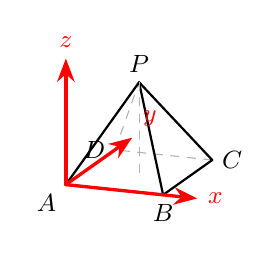
\begin{tikzpicture}[spatial,scale=0.65]
  \coordinate (A) at (0,0,0);
  \coordinate (B) at (2,0,0);
  \coordinate (D) at (0,2,0);
  \coordinate (C) at (2,2,0);
  \coordinate (O) at (1,1,0);
  \coordinate (P) at (1,1,2);
  \draw[dashed,gray!60] (A)--(D)--(C);
  \draw[dashed,gray!60] (D)--(P);
  \draw[thick] (A)--(B)--(C)--(P)--cycle;
  \draw[thick] (B)--(P);
  \draw[dashed,gray!60] (O)--(P);
  \draw[->,red,very thick] (A)--(2.7,0,0) node[right]{\small $x$};
  \draw[->,red,very thick] (A)--(0,2.7,0) node[above right]{\small $y$};
  \draw[->,red,very thick] (A)--(0,0,2.8) node[above]{\small $z$};
  \node[below left] at (A){\small $A$};
  \node[below] at (B){\small $B$};
  \node[right] at (C){\small $C$};
  \node[left] at (D){\small $D$};
  \node[above] at (P){\small $P$};
\end{tikzpicture}
\end{center}
\textbf{建系 A（顶点 $A$ 为原点）}：$P(1,1,2)$，三个分量都非零，计算量较大。
\end{minipage}\hfill
\begin{minipage}[t]{0.48\textwidth}
\begin{center}
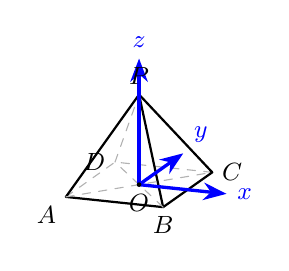
\begin{tikzpicture}[spatial,scale=0.65]
  \coordinate (O) at (0,0,0);
  \coordinate (A) at (-1,-1,0);
  \coordinate (B) at (1,-1,0);
  \coordinate (C) at (1,1,0);
  \coordinate (D) at (-1,1,0);
  \coordinate (P) at (0,0,2);
  \draw[dashed,gray!60] (A)--(D)--(C);
  \draw[dashed,gray!60] (D)--(P);
  \draw[thick] (A)--(B)--(C)--(P)--cycle;
  \draw[thick] (B)--(P);
  \draw[dashed,gray!60] (A)--(C);
  \draw[dashed,gray!60] (B)--(D);
  \draw[dashed,gray!60] (O)--(P);
  \draw[->,blue,very thick] (O)--(1.8,0,0) node[right]{\small $x$};
  \draw[->,blue,very thick] (O)--(0,1.8,0) node[above right]{\small $y$};
  \draw[->,blue,very thick] (O)--(0,0,2.8) node[above]{\small $z$};
  \fill (O) circle (1.3pt) node[below]{\small $O$};
  \node[below left] at (A){\small $A$};
  \node[below] at (B){\small $B$};
  \node[right] at (C){\small $C$};
  \node[left] at (D){\small $D$};
  \node[above] at (P){\small $P$};
\end{tikzpicture}
\end{center}
\textbf{建系 B（推荐：中心 $O$ 为原点）}：$P(0,0,2)$，出现大量零坐标与对称坐标 $\pm1$，方程极易求解。
\end{minipage}
\end{tcolorbox}

\begin{tcolorbox}[colback=white,colframe=rulecolor,boxrule=0.55pt,arc=1mm,title={四、常见几何条件的坐标翻译表},fonttitle=\bfseries]
\begin{tabularx}{\textwidth}{p{3.5cm}Xp{4.2cm}}
\toprule
几何条件 & 向量与坐标转化表达式 & 说明与注意事项 \\
\midrule
中点 $M$ & $\overrightarrow{AM} = \frac{1}{2}\overrightarrow{AB}$ & 坐标取算术平均 $M\left(\frac{x_1+x_2}{2},\frac{y_1+y_2}{2},\frac{z_1+z_2}{2}\right)$ \\ \hline
等长 $PA=PB$ & $\|\overrightarrow{PA}\|^2 = \|\overrightarrow{PB}\|^2$ & 用平方形式展开，避免代数开根号 \\ \hline
垂直 $AB\perp CD$ & $\overrightarrow{AB}\cdot\overrightarrow{CD} = 0$ & 坐标数量积 $x_1 x_2 + y_1 y_2 + z_1 z_2 = 0$ \\ \hline
平行 $AB\parallel CD$ & $\overrightarrow{AB} = \lambda\overrightarrow{CD}$ & $\lambda\neq 0$，写倍数形式避免分母为 $0$ \\ \hline
点 $P$ 在平面 $\alpha$ 内 & $\overrightarrow{AP}\cdot\boldsymbol{n} = 0$ & $A\in\alpha$，$\boldsymbol{n}$ 为平面 $\alpha$ 的法向量 \\
\bottomrule
\end{tabularx}
\end{tcolorbox}

\begin{tcolorbox}[colback=white,colframe=rulecolor,boxrule=0.55pt,arc=1mm,title={五、三类空间角与点面距离公式},fonttitle=\bfseries]
\[
  \cos\theta_{\text{线线}} = \frac{|\boldsymbol{a}\cdot\boldsymbol{b}|}{\|\boldsymbol{a}\|\|\boldsymbol{b}\|},
  \qquad
  \sin\theta_{\text{线面}} = \frac{|\boldsymbol{v}\cdot\boldsymbol{n}|}{\|\boldsymbol{v}\|\|\boldsymbol{n}\|},
  \qquad
  \cos\varphi_{\text{两平面锐角}} = \frac{|\boldsymbol{n}_1\cdot\boldsymbol{n}_2|}{\|\boldsymbol{n}_1\|\|\boldsymbol{n}_2\|}
\]
\[
  d_{\text{点面}} = \frac{|\overrightarrow{AP}\cdot\boldsymbol{n}|}{\|\boldsymbol{n}\|}
\]
\textbf{高频提醒}：向量公式 $\cos\varphi = \frac{|\boldsymbol{n}_1\cdot\boldsymbol{n}_2|}{\|\boldsymbol{n}_1\|\|\boldsymbol{n}_2\|}$ 所求为两平面的\textbf{锐角/直角}。若题目要求求具体的二面角，必须结合图形朝向（法向量方向）判断最终取 $\varphi$ 还是 $\pi-\varphi$。
\end{tcolorbox}

\end{document}